\clearpage
\section{Image reduction}
Calibration frames and science frames have been already taken. Dark frames are not provided and not necessary, since dark currents can be neglected in this case due to proper cooling. Here these images will get inspected and reduced as explained before.
\subsection{Raw-image inspection}
Calibration images are firstly visually inspected using \verb|ds9| with \verb|zscale| setting. Figure~\ref{fig:bias} and~\ref{fig:flat} are examples of bias and flat frames. Note that images shown here are not the whole images.
\begin{figure}[H]
   \centering
   \begin{subfigure}[b]{0.5\textwidth}
   \begin{center}
   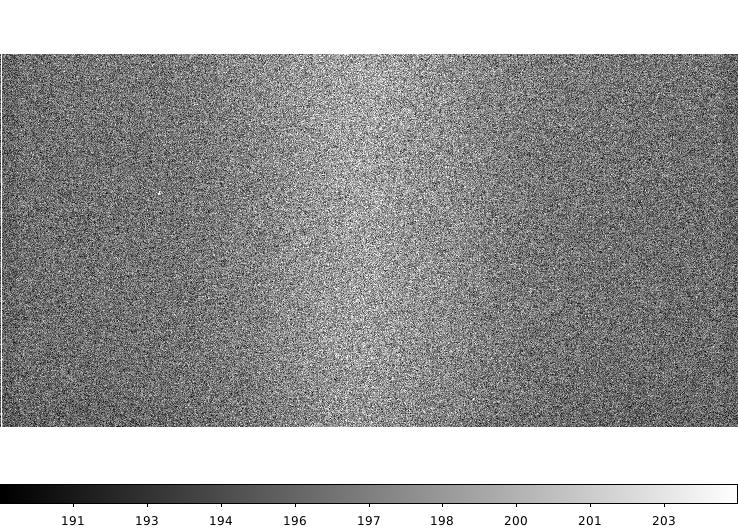
\includegraphics[width=0.8\linewidth]{bias.jpeg}
   \end{center}
   \caption{Bias frame}
   \label{fig:bias}
   \end{subfigure}%
   \begin{subfigure}[b]{0.5\textwidth}
   \begin{center}
   \includegraphics[width=0.8\linewidth]{flat.jpeg}
   \end{center}
   \caption{Flat frame. Color legend was unfortunately not included in screenshot.}
   \label{fig:flat}
   \end{subfigure}
   \caption{Calibration frames. Shown images are only central part of whole images.}%
\end{figure}

Average bias level is somewhat near $200$. This values changes, though not so obvious in figure~\ref{fig:bias}, throughout the image. Left and right sides are significantly darker, meaning less bias. Presumably it is related to geometry and layout of CCD chip. Sometimes one can see quite large white dots in bias picture. Positions of these white dots vary from image to image. Because of its significant size comparing to other noises, they are mostly likely to be cosmic rays, as hinted by~\cite{manual}.

Middle of bias frame is chosen to calculated background and sigma, due to its lack of large-scale variation. Output of \verb|imstats| gives us mean and sigma: $\num{198.72 +- 2.59}$. Noise here should be readout variations and random fluctuations~\cite{manual}.

In flat-field, most obvious feature is black circles or doughnuts. These are dusts on dewar windows and/or filter~\cite{manual}. This results in lower photon counts, thus black in flat-field images. They are not on CCD chips, since they are not properly focused. Some large-scale structure can be seen. It can be explained by different quantum efficiency at different area of CCD. There are quite a lot small sharp black dots visibly. They are most likely to be bad pixels and dust directly on CCD chip.

Each flat-field has different exposure time. One can try to find correlation between mean value of image and exposure time using commands provided in~\cite{manual}. Ratios between these two goes down with increasing exposure time. Firstly of all, CCD chips should be saturated here, since with exposure time, mean values goes down. One possibility is that read-out noise in circuit gets averaged out with long exposure time, thus lower ratio.
\begin{figure}[H]
   \centering
   \includegraphics[width=0.6\linewidth]{mean_exp.pdf}
   \caption{Mean values (red) with sigmas and the ratios (blue) against exposure time of flat-field images.}%
\end{figure}

In science frame one can clearly see doughnut structures and sharp black dots as in flat-field frames. Between exposure, most out-standing change would be that telescope is moving around. 
\begin{figure}[H]
   \centering
   \includegraphics[width=0.8\linewidth]{science.jpeg}
   \caption{An example of science frame.}%
   \label{fig:science}
\end{figure}

We use \verb|image008068.fits| as an example and compute mean and sigma in area without bright objects. Values are \num{693.20 +- 19.00}. It is greater than the mean value of bias frame. This is easy to understand, since science frame must contain sky. 

\subsection{Image reduction}
Several science frames containing source \verb|SDSS1650+4251|  are taken from one filter ($R$). Now these images with be reduced with help of calibrations frames and some more in \verb|theli|. \verb|theli| mainly consists of several tabs or processing groups. Each of following paragraph corresponds one processing group/

\paragraph{Initialise}  First off, \verb|theli| should be properly reset and initialised. Number of CPU cores and instrument (telescope) are specified accordingly. Paths containing bias, flat, and science frames are filled in.

\paragraph{Preparation}
Through this processing group, headers contained in \verb|.fits| files can be split and/or corrected. Comparison of headers before and after corrections reveals
\begin{itemize}
   \item size in $x$ and $y$ are swapped, meaning orientation of images has been changed,
   \item (useless) information, e.g.~comments, CCD info, Date, and etc., has been removed,
   \item lots of lines starting with \verb|DUMMY| have been added.
\end{itemize}
They are more changes, but the listed alterations are most noticeable.

\paragraph{Calibration}
In this step, calibration frames are getting co-added. In co-addition process, images are stacked on top of each other, while making sure each object falls onto the same pixel~\cite{manual}. By doing this and in the end only calibrating with co-added images, random noises will get averaged out.  

After co-addition, bias frames are free of small white dots as seen before and flat frames get a bit brighter. One can further computer noise dispersion of co-added bias frame and single bias frame. They are respectively \num{0.72} and \num{2.27}. So noise level in co-added images is much lower.

The minimal value in normalised flat-field is $0$. Dithering during co-addition helps to remove bright objects (stars and etc.).

\paragraph{Background modelling}
In this processing group, only background model correction is selected, where a superflat and fringe model is created and applied. Its configurations are set according to~\cite{manual}: $\verb|DT| = 1.0$, $\verb|DMIN|=10$, mask expansion factor$=3$, \verb|median| combination, \verb|divide smoothed model, subtract fringes| method, smoothing kernel for background model $=256$.

In superflat, one can clearly see fringes pattern. Fringes and background sky can be extracted with smoothing process. In \verb|SDSS1650+4251_R_block0_1_fringe.fits|, there is only fringes visible and in \verb|SSD1650+4251_R_block0_1_illum.fits| only smooth gradient, i.e.~background.

Correction given by illumination is roughly \num{500} (counts). Fringes are removed after correction, see figure~\ref{fig:before} and~\ref{fig:after}.
\begin{figure}[H]
   \centering
   \begin{subfigure}[t]{0.5\textwidth}
   \begin{center}
   \includegraphics[width=\linewidth]{before.jpeg}
   \end{center}
   \caption{Before correction. Pay attention to top left corner.}
   \label{fig:before}
   \end{subfigure}%
   \begin{subfigure}[t]{0.5\textwidth}
   \begin{center}
   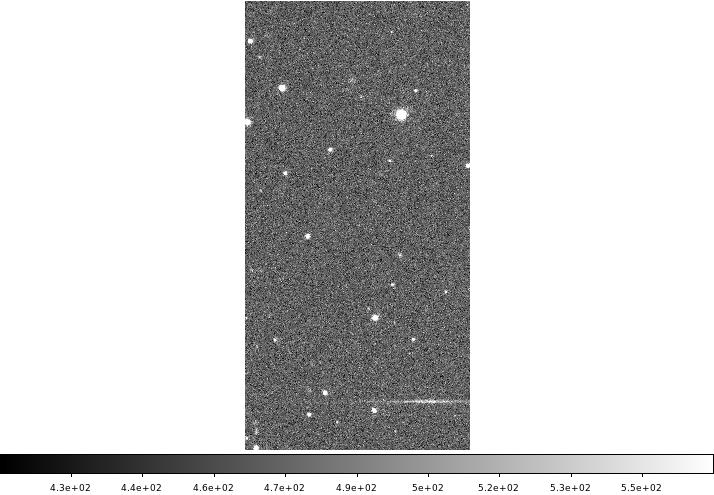
\includegraphics[width=\linewidth]{after.jpeg}
   \end{center}
   \caption{After correction. Pay attention to top left corner.}
   \label{fig:after}
   \end{subfigure}
\end{figure}

\paragraph{Weighting} 
In this step, weighting and masking are performed to compensate bad pixels and different quantum efficiency. Global weights and WEIGHTS are created and applied.

\paragraph{Astrometry/Photometry}

\paragraph{Co-addition}


\section{PSF extraction}

\section{Component fitting}

\section{Time-delay estimate}

\section{Lensing analysis}
